\documentclass[12pt]{article}
\setlength{\evensidemargin}{5pt}
\setlength{\marginparwidth}{0pt}
\setlength{\marginparsep}{0pt}
\setlength{\textheight}{9in}
\setlength{\tabbingsep}{0pt}
\setlength{\headsep}{30pt}
\setlength{\fboxsep}{40pt}
\setlength{\fboxrule}{4pt}
\setlength{\footnotesep}{20pt}
\setlength{\parindent}{0pt}
\setlength{\parskip}{8pt plus 5pt}
\setlength{\topmargin}{-0.5in}
\setlength{\oddsidemargin}{0in}
\setlength{\textwidth}{6.5in}

\usepackage{times}
\usepackage{url}
\usepackage{graphics}
\usepackage{graphicx}      % extended graphics package
\usepackage{epsfig}        % wrapper for graphicx package
\usepackage[noend]{algpseudocode}
\algrenewcommand\algorithmicprocedure{\textbf{ALGORITHM}}

\begin{document}

\title{An Empirical Study of the Brute-Force Closest Pairs Algorithm}

\author{Jim Teresco\\
jteresco@siena.edu\\
\and
My Partner\\
partner@fake.email}

\maketitle

\begin{abstract}
  In this study, which is intended as an example of how to put
  together the writeup for an empirical study of algorithm
  performance, we present and analyze timings and operation counts for
  a straightforward brute-force closest pairs implementation.  Points
  are generated randomly in a specified range, and the closest pair is
  computed and reported by a Java program.
\end{abstract}

\section{Introduction}

This empirical analysis study focuses on the brute-force closest pairs
algorithm in two dimensions.  We will consider a straightforward
implementation of the algorithm in Java, instrumented to count basic
operations and gather timings.

The remainder of this report is organized as follows.
Section~\ref{sec:environment} describes the computing environment
used.  Section~\ref{sec:bfcp} describes the algorithm, our
expectations based on the theoretical analysis, presents our results,
and relates them back to the theory.  We conclude with some additional
discussion in Section~\ref{sec:conclusions}.

\section{Computing Environment}
\label{sec:environment}

For this study, a Java program was developed that implements the
algorithm of interest.  Random inputs of varying sizes and other
characteristics are generated, and the solution is computed.

All runs are using the following Java version:

\begin{verbatim}
java version "1.8.0_121"
Java(TM) SE Runtime Environment (build 1.8.0_121-b13)
Java HotSpot(TM) 64-Bit Server VM (build 25.121-b13, mixed mode)
\end{verbatim}

The computing environment is a MacBook Pro (15-inch, 2016) with a 2.6
GHz Intel Core i7, 16 GB of 2133 MHz LPDDR3 memory, and running macOS
Sierra Version 10.12.6.  There are 4 cores, each with 256 KB L2 cache,
and these cores share a 6 MB L3 cache.

\section{Brute-Force Closest Pairs}
\label{sec:bfcp}

The brute-force closest pairs algorithm as shown in
Figure~\ref{fig:alg} was implemented in Java, and instrumented to
count the number of times the distance between pairs of points is
computed and to report the elapsed time for the main loops to execute.

\begin{figure}[htb]
  \centering
\begin{algorithmic}
  \Procedure{BruteForceClosestPoints}{$P$}
  \State //Input: a set of points $P[0..n-1]$
  \State $d_{min} \gets \infty$
  \For{$i \gets 0 .. n-2$}
  \For{$j \gets i+1 .. n-1$}
  %\State $d \gets distance(P[i], P[j])$
  \State $d \gets \sqrt{(P[i].x - P[j].x)^2 +(P[i].y - P[j].y)^2}$
  \If {$d < d_{min}$}
  \State $d_{min} \gets d$
  \State $index_1 \gets i$
  \State $index_2 \gets j$
  \EndIf
  \EndFor
  \EndFor
  \State \textbf{return} $(index_1, index_2)$
\EndProcedure
\end{algorithmic}
\caption{The brute-force closest pairs algorithm, as implemented for
  this study.}
\label{fig:alg}
\end{figure}

The number of points for the runs is all powers of 2 from
$2^{10}=1024$ to $2^{19}=524,288$.  Points for each run are generated
randomly, within a range specified as a parameter to the program.
Points are generated within the square with x- and y-coordinates no
further than that range from the origin.

Each combination of the number of points and range of point positions
is run a total of 5 times.  The number of distance calculations is
expected to be identical for each of the runs for a given number of
points.  Run times will vary, however, and the minimum time for a
given combination of the number of points and range of point positions
is chosen to minimize the effects from other computations that could
be in process on the computer during the study.


\subsection{Expectations}

The theoretical expectation is for both the number of distance
calculations and elapsed time to be $\Theta(n^2)$ in the best,
average, and worst cases.  There are no shortcuts out of the loops,
which execute about $\frac{n^2}{2}$ times.

\subsection{Results}

The raw results of the study are available in the file
\texttt{timings.dat} in the GitHub repository.  Each line, such as

{\small
\begin{verbatim}
BFCP 262144 64.0 92375.0 34359607296 (99936,203911) 4.069483000753879E-4
\end{verbatim}
}

has 7 space-separated fields.  The first field indicates the algorithm name,
and is followed by the number of points, the range of coordinate
values (each of x and y are within this distance of the origin), the
elapsed time in milliseconds, the number of distance calculations, the
indices of the two points that were found to be the closest pair, and
the distance between those points.  Of these, we are interested in the
number of points, the elapsed time, and distance calculation count.

\begin{figure}[htb]
  \centering
  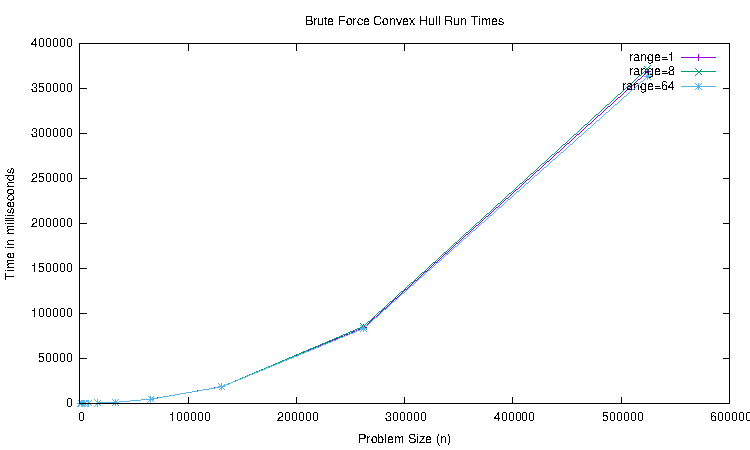
\includegraphics{bfcp-times.pdf}
  \caption{Times in milliseconds for the brute-force closest pairs to
    complete its computation for problem sizes from $2^{10}$ to
    $2^{19}$ points.}
  \label{fig:timings}
\end{figure}

\begin{figure}[htb]
  \centering
  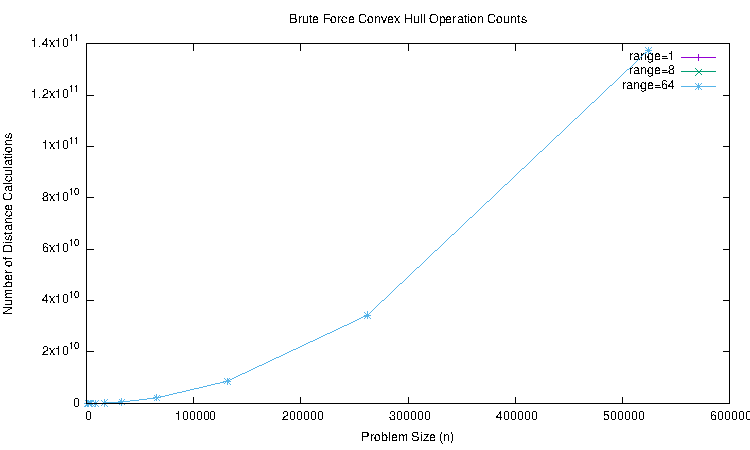
\includegraphics{bfcp-opcounts.pdf}
  \caption{Number of distances between pairs of points computed the
    brute-force closest pairs to complete its computation for problem
    sizes from $2^{10}$ to $2^{19}$ points.}
  \label{fig:opcounts}
\end{figure}

\begin{table}[htb]
  \centering
  \begin{tabular}{|c|c|c|}
    \hline
    Problem Size & Time (ms) & Distance Calculations \\ \hline \hline
1024 & 11.0 & 523776 \\ \hline
2048 & 15.0 & 2096128 \\ \hline
4096 & 35.0 & 8386560 \\ \hline
8192 & 81.0 & 33550336 \\ \hline
16384 & 298.0 & 134209536 \\ \hline
32768 & 1171.0 & 536854528 \\ \hline
65536 & 4607.0 & 2147450880 \\ \hline
131072 & 18496.0 & 8589869056 \\ \hline
262144 & 84123.0 & 34359607296 \\ \hline
524288 & 368682.0 & 137438691328 \\ \hline
  \end{tabular}
  \caption{Actual times and operation counts used to create the plots
    in Figure~\ref{fig:timings} and Figure~\ref{fig:opcounts}.}
  \label{tab:rawdata}
\end{table}

Figure~\ref{fig:timings} shows the times in milliseconds (minimum
across 5 runs of each) and Figure~\ref{fig:opcounts} shows the number
of computations of the distance between two points for this study.
Unsurprisingly, the timings are very similar and the operation counts
identical for the different ranges of point placements, so
Table~\ref{tab:rawdata} shows the data as plotted in the figures but
only for the range value of 1.0.

\subsection{Discussion}

Both the timings and distance calulation counts match well with the
expected $\Theta(n^2)$ behavior of this algorithm.  The graphs in
Figures~\ref{fig:timings} and~\ref{fig:opcounts} show the expected
parabolic shape.  The actual numbers in Table~\ref{tab:rawdata} align
well.  The number of distance calculations is exactly as predicted.
Any variation there would have indicated an error in the algorithm or
in the instrumentation that counted the operations.  For the timings,
small problem sizes are subject to errors due to the accuracy of the
millsecond timer over short timespans.  However, when we look at the
larger problem sizes, we see exactly what we would expect: when we
double the problem size, the time taken to compute the solution
increased by a factor of four.

\section{Conclusions}
\label{sec:conclusions}

In this simple study, we found that all of our results matched the
expected behavior from the theory.  In this particular algorithm,
since there are no asymptotic differences among the best-, average-,
and worst-case behavior, this should be unsurprising.  The small
variations in run time can perhaps be explained by how soon the
algorithm finds the closest pair (or at least a very close pair).  The
more times that a new closest pair is found, the more often the body
of the \texttt{if} statement following the distance calculation will
need to execute.  There is also the issue that the computer used for
the study is a laptop system that had many processes such as web
browsers with many tabs and terminal windows in regular interactive
use during the timing studies.  This is partially accounted for by
taking the minimum time across 5 runs, but as each run has its own set
of random points generated, the previously-mentioned effect from the
different numbers of times the body of the \texttt{if} statement is
executed will potentially skew the results more toward a best case
behavior.  Any such variations are likely minor, and do not decrease
the confidence in our conclusions that the timing results match
closely with theoretical expectations.

\end{document}
